%! suppress = LineBreak
\documentclass[prd,twocolumn,tightenlines,preprintnumbers,showpacs,superscriptaddress,notitlepage,nofootinbib,eqsecnum,floatfix,longbibliography,aps,10pt]{revtex4-2}
\usepackage{CJK}
\usepackage[utf8]{inputenc}
\usepackage[T1]{fontenc}
\usepackage{amsmath}
\usepackage{mathtools}
\usepackage{amsfonts,dsfont}
\usepackage{bm,bbm}
\usepackage{graphicx}
\usepackage{xcolor}

\usepackage{hyperref}
\hypersetup{
    colorlinks=true,     % false: boxed links; true: colored links
    linkcolor=blue,      % color of internal links
    citecolor=blue,      % color of links to bibliography
    filecolor=blue,      % color of file links
    urlcolor=blue        % color of external links
}

% disable subsections and subsubsections in the TOC
\makeatletter
\def\l@subsubsection#1#2{}
\makeatother


\begin{document}
\title{Solutions to Integer Programming from Quantum Annealing}

\author{Chia~Cheng~Chang}
\affiliation{RIKEN iTHEMS, Wako, Saitama 351-0198, Japan}
\affiliation{Department of Physics, University of California, Berkeley, California 94720, USA}
\affiliation{Nuclear Science Division, Lawrence Berkeley National Laboratory, Berkeley, California 94720, USA}
	\author{Chih-Chieh~Chen }
\affiliation{R\&D Group, Grid Inc., Tokyo 107-0061, Japan}
\affiliation{Department of Physics, University of California, Berkeley, California 94720, USA}
\author{Christopher K\"orber}
\affiliation{Institut f\"ur Theoretische Physik II, Ruhr-Universit\"at Bochum, D-44780 Bochum, Germany}
\affiliation{Department of Physics, University of California, Berkeley, California 94720, USA}
\author{Travis~Humble}
\affiliation{Quantum Computing Institute, Oak Ridge National Laboratory, Oak Ridge, Tennessee 37831, USA}
\affiliation{Computational Sciences and Engineering, Oak Ridge National Laboratory, Oak Ridge, Tennessee, 37831, USA}
\author{Jim~Ostrowski}
\affiliation{Industrial and Systems Engineering, University of Tennessee, Knoxville, Tennessee 37996, USA}

\newcommand{\alert}[1]{\textbf{\color{red}{#1}}}
\renewcommand{\vec}[1]{\boldsymbol{#1}}

\newcommand{\ghissue}[2]{
 \noindent\fbox{\parbox{0.49\textwidth}{
   \alert{[#1]}%
   \\%
   \href{https://github.com/cchang5/quantum\_linear\_programming/pull/#2}{See GitHub issue #2}}%
 }
}


\begin{abstract}
 While quantum computing proposes promising solutions to computational problems not accessible with classical approaches, due to current hardware constraints, most quantum algorithms are not yet capable of computing systems of practical relevance, and classical counterparts outperform them.
 To practically benefit from quantum architecture, one has to identify problems and algorithms with favorable scaling and improve on corresponding limitations depending on available hardware.
 For this reason, we developed an algorithm that solves integer linear programming problems (ILP), a classically NP-hard problem, on a quantum annealer (QA), and investigated problem and hardware-specific limitations.
 This work presents the formalism of how to map ILP problems to the annealing architectures, how to systematically improve computations utilizing optmizied anneal schedules and models the anneal process through a simmulation.
 It illustrates the effects of decoherence and Many-Body Localization, for the Minimum Dominating Set problem, and compares annealing results against numerical simulations of the quantum architecture.
 We find that the QA ILP algorithm outperforms random guessing but is limited to small problems and that annealing schedules can be adjusted to reduce the effects of decoherence.
 Simulations qualitatively reproduce algorithmic improvements of the modified annealing schedule, suggesting the improvements have origins from quantum effects.
\end{abstract}

\preprint{RIKEN-iTHEMS-Report-20}

\maketitle
%%%%%%%%%%%%%%%%%%%%%%%%%%%%%%%%%
%%%%%%%%%%%%%%%%%%%%%%%%%%%%%%%%%
%%%%%%%%%%%%%%%%%%%%%%%%%%%%%%%%%
%\tableofcontents

\flushbottom
\maketitle

%========================================================================================
\section{INTRODUCTION}
\label{sec:introduction}
%========================================================================================

Integer Linear Programming (ILP) is an integer optimization problem subject to inequality constraints
\begin{align}
 \label{eq:initial-ip-def}
 \vec x_0 = \mathrm{arg} & \min\limits_{x}\left(\sum_i c_i x_i\right)
\end{align}
subject to
\begin{align}
 \label{eq:ilp-constraints}
  & \sum_i A_{ai}x_i +b_a \leq 0 \,, \\
  & x_i  \in \mathbbm{Z} \geq 0\, ,
\end{align}
where $i=1, \cdots,  N$ is the number of dependent variables and $a=1, \cdots, M$ the number of constraint equations.

ILP is a commonly tackled problem applicable to situations such as x~\cite{}, y~\cite{}, and the Minimum Dominating Set Problem (MDS)~\cite{}.
In general, ILP is classically NP-complete, and as a result, heuristic methods are employed~\cite{}.
Standard classical heuristic algorithms employ a greedy scheme which iteratively approximates optimal solutions--starting from a random initial guess, these algorithms apply locally optimal choices at each step.
The NP-hardness of ILP can be understood by realizing that while the solution to an $n$-dimensional linear problem can be obtained in polynomial time, the optimal integer solution in general must be found in the $2^n$ integer solutions which surround the real number solution.
While greedy algorithms do not guarantee optimal global solutions, they find approximate solutions in polynomial time, which can be utilized in further computations.

An important ILP application is the Minimum Dominating Set problem, which is representatively considered in this work.
For a given a graph $G(E,V)$, defined by the set of $V$ vertices and $E$ edges, a dominating set $D$ is a specific subset of vertices $D \subseteq V$.
In particular, $D$ is a dominating set if all vertices in $V$ but not in $D$ are adjacent to at least one vertex in $D$.
This is equivalent to requiring the set of nearest-neighbor vertices of $D$ (exclusive) and $D$ cover all vertices $N(D) \cup D = V$ (an example is given by Fig.~\ref{fig:dominating_sets}a).
The set $D$ is a minimal dominating set if there is no proper subset of $D$ that is a dominating set, {\it{i.e.}}, the removal of any vertex in $D$ results in $N(D) \cup D  \neq V$.
An example is given by Fig.~\ref{fig:dominating_sets}b.
The domination number of $D$ is given by the cardinality of $|D| \equiv \overline{\overline{D}}$.
The Minimum Dominating Set (MDS) is defined by $D$ with the smallest domination number.
Fig.~\ref{fig:dominating_sets}c shows an example of the minimum dominating set of $G(V, E)$ and is different from the minimal dominating set.
We emphasize that while the maximum independent set is always a minimal dominating set as exemplified by Fig.~\ref{fig:dominating_sets}b, the minimum dominating set, in general, can have a smaller domination number.
As a result, the solution to the dominating set problem can not be obtained by solving for the maximum independent set, a well-studied problem for quantum annealers~\cite{}.

\begin{figure*}
	\centering
	\begin{tabular}{p{0.2\textwidth}p{0.1\textwidth}p{0.2\textwidth}p{0.1\textwidth}p{0.2\textwidth}}
	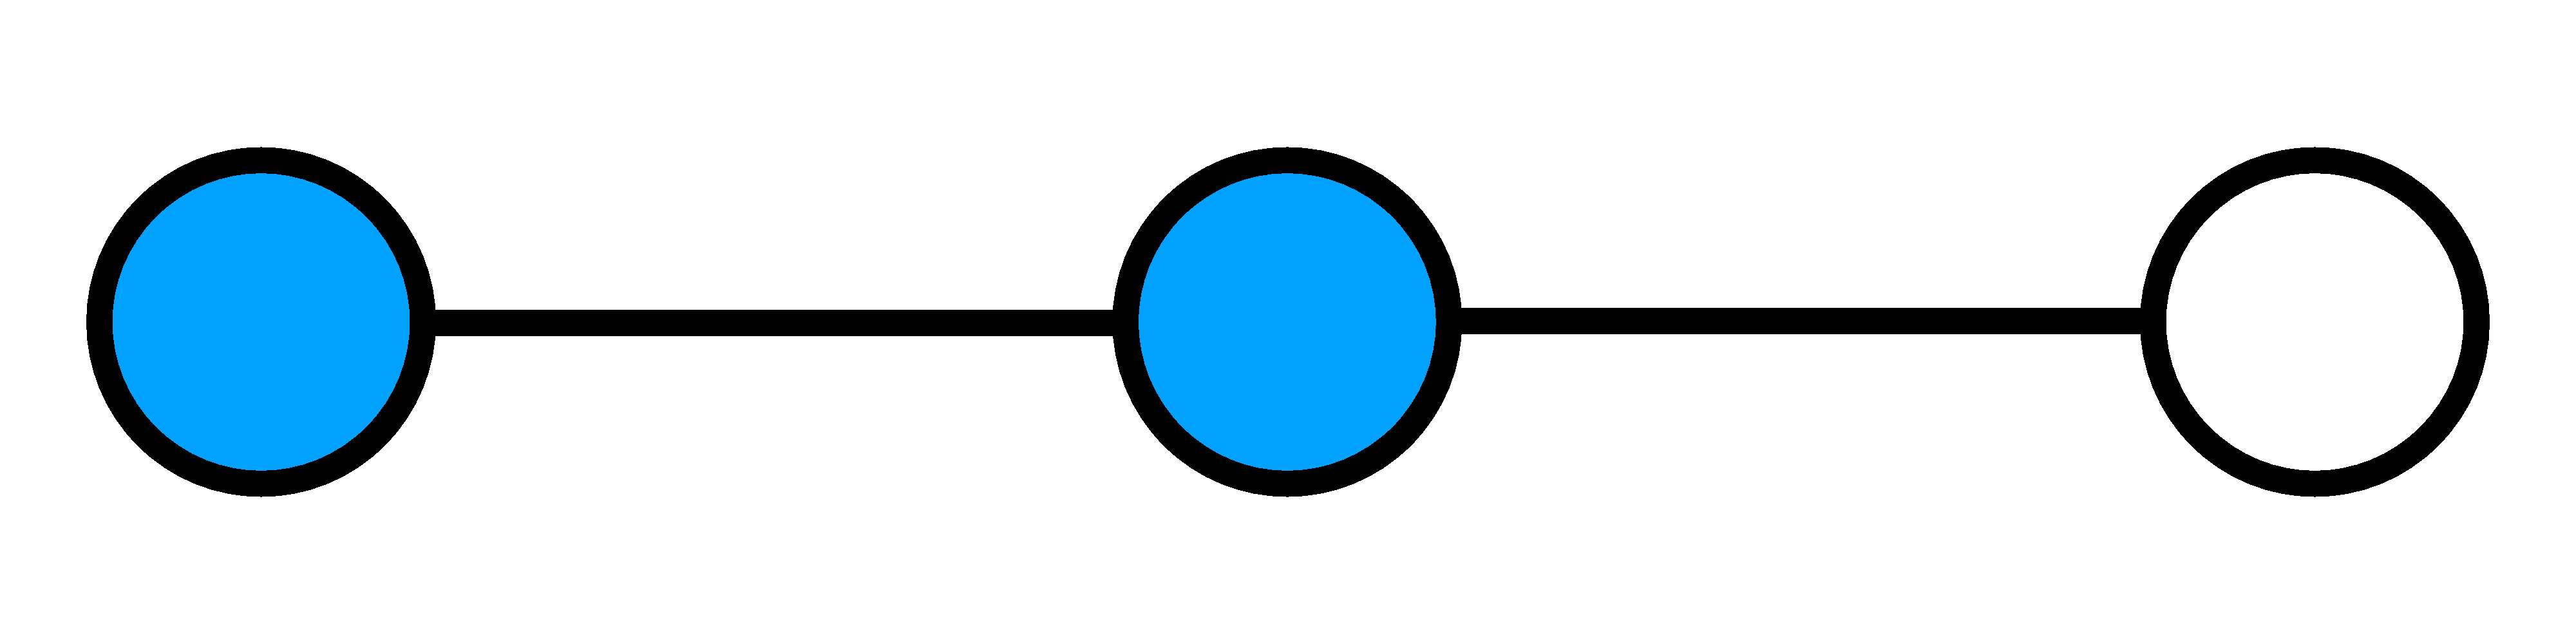
\includegraphics[width=0.2\textwidth]{./new_figures/MDS_mds0.pdf}
&&
	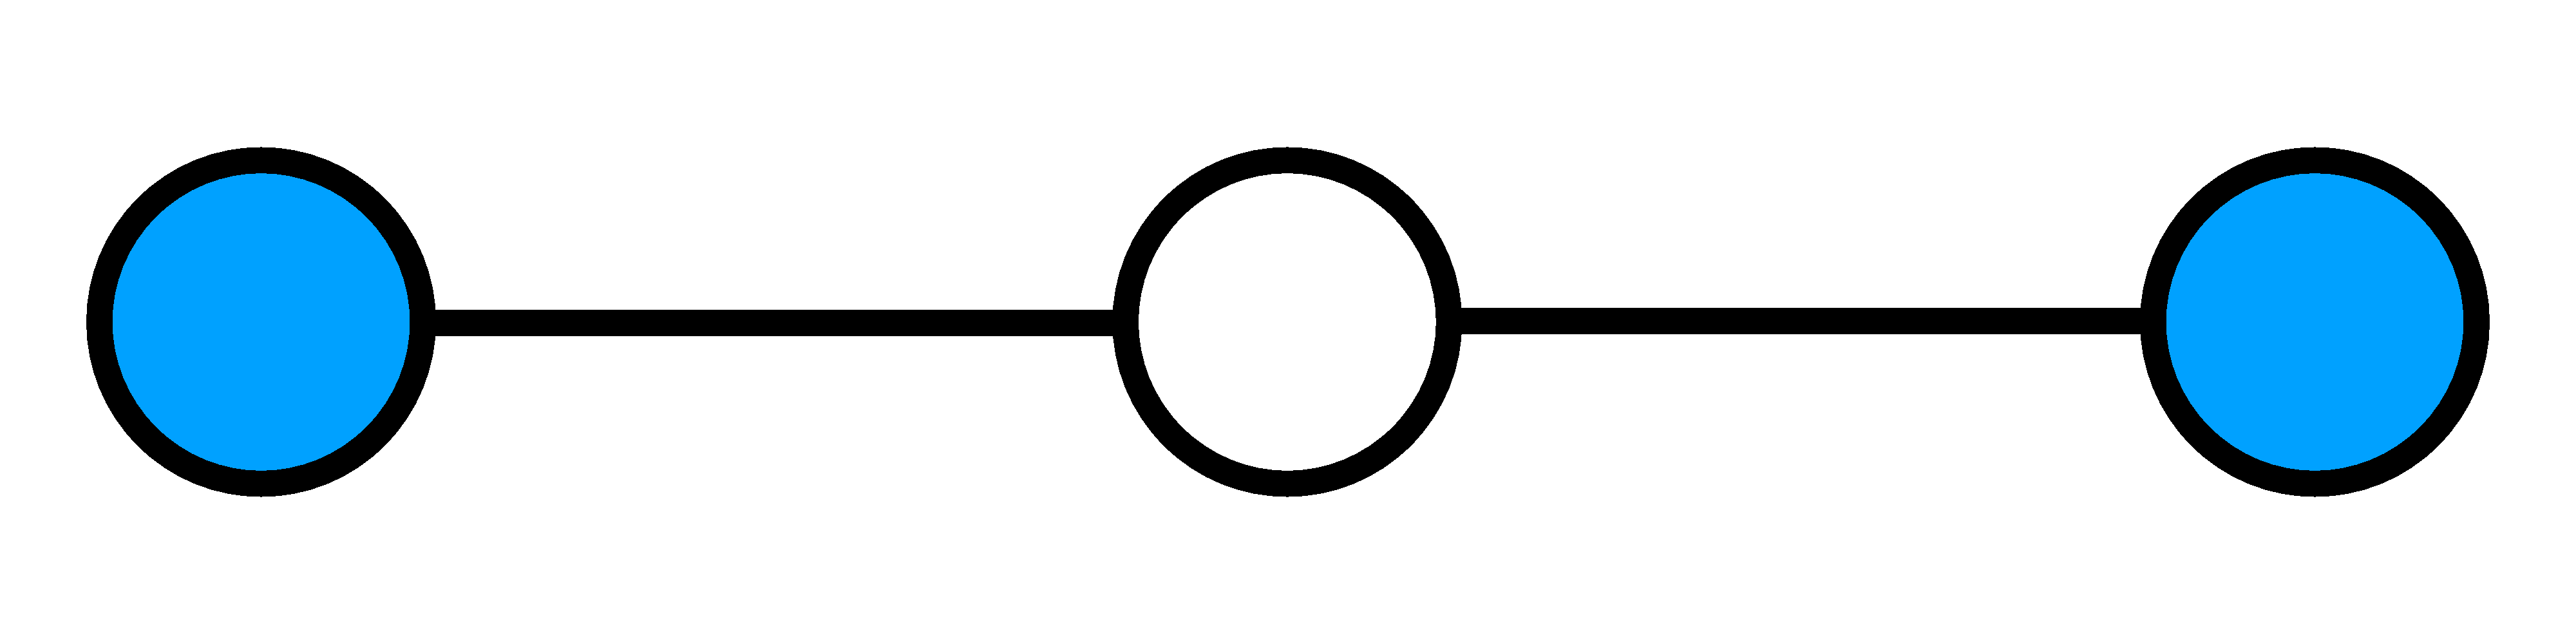
\includegraphics[width=0.2\textwidth]{./new_figures/MDS_mds1.pdf}
&&
	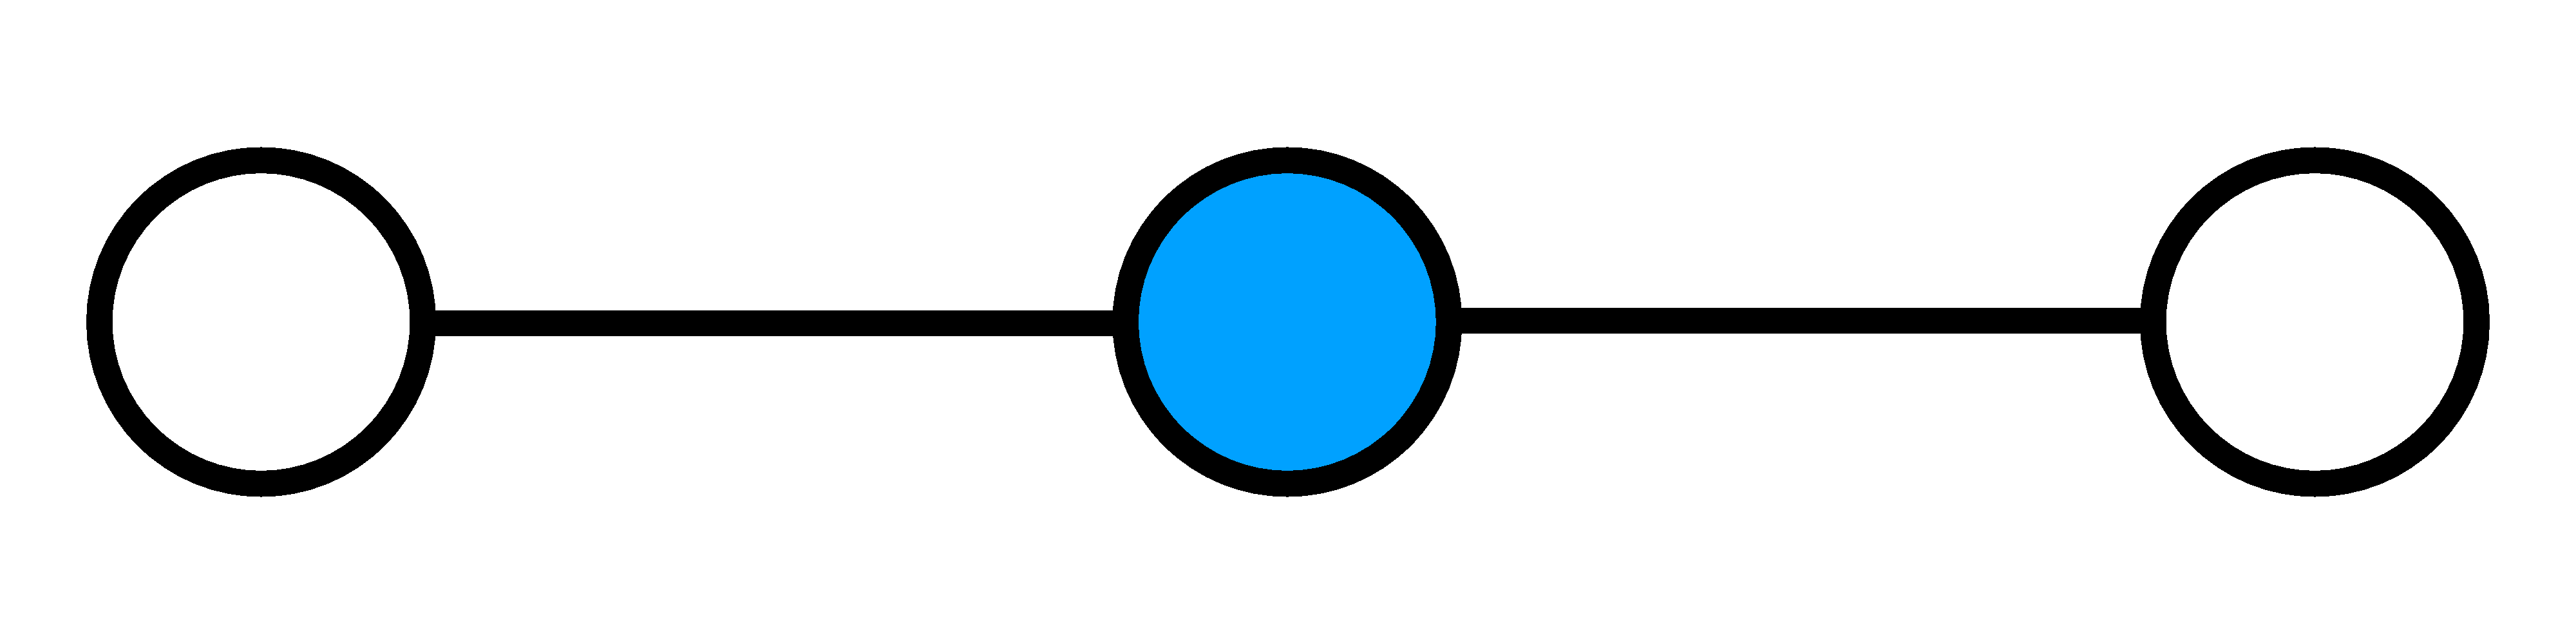
\includegraphics[width=0.2\textwidth]{./new_figures/MDS_mds2.pdf}\\
	\centering\bf{a} && \centering\bf{b} && \centering\bf{c}
	\end{tabular}
	\caption{Example of different dominating sets for $G(V, E)$. Vertices in the dominating set $D$ are highlighted in blue. {\bf{a)}} A dominating set of $G$ with domination number $\overline{\overline{D}} = 2$. {\bf{b)}} A minimal dominating set of $G$ with domination number of $\overline{\overline{D}} = 2$. {\bf{c)}} The minimum dominating set of $G$ with domination number of $\overline{\overline{D}} = 1$.}
	\label{fig:dominating_sets}
\end{figure*}

For general graphs, existing algorithms on classical computers find MDS solutions in exponential time $\sim O( 1.5^n)$ \cite{Fomin2009, vanRooij2009} or approximate solutions in polynomial time. For example, greedy algorithms locally optimize decisions about which nodes to add to the dominating set.
Thus one is guaranteed to find a dominating set but not necessarily an MDS.

Due to the importance and difficulty in this work, we present a method to obtain optimal solutions to ILP by employing quantum annealing methods.

Quantum annealing solves a general quadratic binary optimization problem (QUBO) by slowly varying a time-dependent Hamiltonian~\cite{}.
Through the adiabatic theorem of quantum mechanics, the annealer is initially prepared in a trivial ground state while the final Hamiltonian encodes the solution to the ILP.
Due to the explosion in research efforts towards hardware implementations of quantum annealers and future improvements to the annealing schedule~\cite{}, mapping ILP to QUBO provides a path forward towards obtaining optimal solutions to the class of integer optimization problems~\cite{2018Glover}.

A quantum annealer evolves the ground state of an initial Hamiltonian into the problems Hamiltonian's ground state by adiabatically changing the hardware that implements Hamiltonian.
Thus, the implemented Hamiltonian is explicitly time dependent
\begin{equation}
 H(t) = A(t) H^{\textrm{init}} + B(t) H^{\textrm{problem}}, \label{eq:tdhamiltonian}
\end{equation}
and $H^\textrm{init}=\sum_i\sigma^x_i$ on the DWave, while $H^\textrm{problem}$ encodes the problem to be solved.

In this paper, we propose an algorithm that maps ILP problems to QUBO.
This is achieved by the introduction of slack variables $s$ which turn the inequalities eq.~\eqref{eq:ilp-constraints} to equalities
\begin{align}
  \label{eq:ilp:slack}
  & \sum_i A_{a i}x_i + s_a + b_a = 0, \\
  & x_i, s_a \in \mathbb{Z} \geq 0.
\end{align}
While the coefficients of the inequality constraints are not required to be integer valued, the inequalities can be trivially rescaled such that $s_i \in \mathbbm{Z}$ given fixed precision coefficients $A_{ij}$ and $b_i$.
Furthermore, this formalism can be generalized to constrained quadratic optimizations \ref{sec:methods:ilp:quadratic}.

We further improve the quantum annealer's performance by utilizing annealing offsets, which effectively delays the annealing schedule on a per-qubit basis. \cite{PhysRevA.96.042322,hsu2018quantum,10.1007/978-3-030-14082-3_14}
Converting to the Ising representation of the the problem Hamiltonian,
\begin{equation}
    \label{eq:HIsing}
     H^{\textrm{Ising}} = \sum_{ij} J_{ij} \sigma^z_i \sigma^z_j + \sum_i h_i \sigma^z_i ,
\end{equation}
we can recognize that Eq.~(\ref{eq:HIsing}) exhibits spin-glass properties. More specifically, if the $h_i$ coefficients are randomly drawn from a Bernoulli distribution, one expects spin-localization behavior to influence the outcome of the anneal.
In the case of quantum annealing, when an algorithm is mapped to its Ising representation, the values of $h_i$ will frequently take on various values, mimicking spin-glass like behavior.
More explicitly, the spin-glass enters a glassy state when more disorder is introduced ($|h_i|$ becomes large), and as a consequence, the wavefunction experiences Many-Body Localization (MBL) effects, the many-body analog of Anderson Localization~\cite{doi:10.1146/annurev-conmatphys-031214-014726,PhysRevE.90.022103,RevModPhys.91.021001}.
dd

Our improvement strategy is motivated by the MBL hypothesis.
That is, we want the system to be ergodic and avoid the MBL phase.
As a result, we employ a modified annealing schedule which relies on partitioning the Hamiltonian into regions of relatively weak and strong external magnetic fields~\cite{doi:10.7566/JPSJ.89.044001}.


To understand which phenomena are relevant for describing the proposed offset study's scaling behavior, whether they are rooted in the quantum nature or related to hardware constraints, we simulate the anneal for a small MDS problem. This simulation solves the von Neumann equations accounting for different models of quantum decoherence, and explores whether algorithmic improvements on hardware are present in idealizes systems.


%========================================================================================
\section{RESULTS}
\label{sec:results}
%========================================================================================

We first present the QUBO mapping for ILP (\ref{sec:results:qa1}), and demonstrate the methodology on an example implementation in case of the Minimal Dominating Set problem (\ref{sec:results:qa}) on the DWave quantum annealer. Results from quantum annealing are compared and discussed in contrast to simulations (\ref{sec:results:simulation}).

%----------------------------------------------------------------------------------------
\subsection{ILP QUBO}
\label{sec:results:qa1}
%----------------------------------------------------------------------------------------
Following Eq.~(\ref{eq:ilp:slack}), the ILP problems simplifies to solving a system of linear equations on integer valued variables. We map the integer variables $\vec z = \vec x, \vec s$ appearing in eq.~\eqref{eq:ilp:slack} to qubits under the following transformation~\cite{Chang:2018uoc}
\begin{align}
 z_i = & \sum_{r=0}^{R_i-1} 2^r \psi_{ri}
 \label{eq:int_to_bin}
\end{align}
where $\psi_{ri} \in \{0, 1\}$. The number of qubits used to represent the $i$-th integer variable is allowed to vary with $R_i$.
The integer-vector qubit transformation can be expressed as a rectangular matrix.
For example, a vector of two integer variables $z_0$ and $z_1$ represented by one and two qubits respectively is given as
\begin{align}
 \begin{pmatrix}
  z_0 \\
  z_1
 \end{pmatrix}
 = &
 \begin{pmatrix}
  2^0 & 0   & 0   \\
  0   & 2^0 & 2^1
 \end{pmatrix}
 \begin{pmatrix}
  \psi_{00} \\
  \psi_{01} \\
  \psi_{11}
 \end{pmatrix}
 \equiv T^z \begin{pmatrix}
  \psi_{00} \\
  \psi_{01} \\
  \psi_{11}
 \end{pmatrix}
\end{align}
If all variables are represented by the same number of qubits--$R_i$ is a constant for all $i$--then one can express the transformation as tensor product of bit vectors
\begin{align}
 \mathcal{R} =  & \begin{pmatrix} 2^0 & \dots & 2^{R-1}\end{pmatrix},    \\
 \mathcal{Z} =  & \begin{pmatrix} z_0 & \dots & z_{N-1}\end{pmatrix},    \\
 |\mathds{1}| = & |\mathcal{Z}|,                 \\
 T^z =          & \mathds{1}\otimes \mathcal{R}.
\end{align}

As a result, the $\vec x$ and $\vec s$ map to the binary vector $\vec \Psi$ under the transformation
\begin{equation}
    \begin{pmatrix}
        \vec x \\ \vec s
    \end{pmatrix}
    =
    \begin{pmatrix}
        T_x & 0 \\ 0 & T_s
    \end{pmatrix}
    \begin{pmatrix}
        \vec \Psi_x \\ \vec \Psi_s
    \end{pmatrix}
    =
    T
    \vec \Psi
\end{equation}

The integer linear optimization problem is then solved through the minimization of the quadratic objective function
\begin{align}
 \chi^2(\vec \Psi)
 &=
 \vec c^T T_x \vec \Psi_x + p \left\| A T_s \vec \Psi_x + T_s \vec \Psi_s + \vec b \right\|^2
\end{align}
where $p$ is an external parameter representing the strength of the penalty when violating constraints.
This parameter needs to be sufficiently large, e.g., $p \geq \vec c \cdot \vec x$, to ensure the constraints are indeed fulfilled\footnote{Depending on the problem, $p$ can be smaller as well.
For example, in the case of the MDS, $p\geq 1$ suffices.}.
The objective function $\chi^2$ can be represented as a QUBO Hamiltonian
\begin{align}
 \chi^2(\vec \Psi) =    &
 \vec \Psi^T
 \begin{pmatrix}
  Q_{xx} & Q_{xs} \\
  Q_{sx} & Q_{ss}
 \end{pmatrix}
 \vec \Psi + p\left \| \vec b \right\|^2, \\
 \equiv &  \vec \Psi^T Q  \vec \Psi + C,
 \label{eq:matrix_form}
\end{align}
where
{\small
\begin{align}
 \label{eq:qubo:components}
 Q_{xx} = & p {T_{x}}^T \left[ A^T A + \mathrm{diag} \left(A^T \vec b + \vec b^T A\right) \right] T_x + \mathrm{diag}(\vec c) T_x,                                                                    \\
 Q_{xs} = & Q_{sx}^T = p {T_{x}}^T A^T T_s,                                                                     \\
 Q_{ss} = & p\left[ {T_{s}}^T T_s + \mathrm{diag}\left( {T_{s}}^T \vec b + \vec b^T T_s\right) \right].
\end{align}}
The function $\mathrm{diag}(\vec v)$ transforms a vector $\vec v$ into a diagonal matrix, and absorbs the linear contributions of the QUBO into the diagonal elements of the quadratic representation.

The integer solution to the original ILP is computed by $\vec x^{(0)} = T_x \vec \Psi_x^{(0)}$ and the original solution to the problem is computed by shifting the annealer extracted energy $E \equiv  \chi^2(\vec \Psi^{(0)}) $ by $p \left \| \vec b \right\|^2$.
The slack components of this vector $\vec \Psi_s$ can be utilized to check if the contraints are indeed fulfilled.

%----------------------------------------------------------------------------------------
\subsection{Dominating Set scaling \& offset study}
\label{sec:results:qa}
%----------------------------------------------------------------------------------------
\begin{figure}[b]
	\centering
	\begin{tabular}{cc}
	$G(n):$ &
	\raisebox{-.4\height}{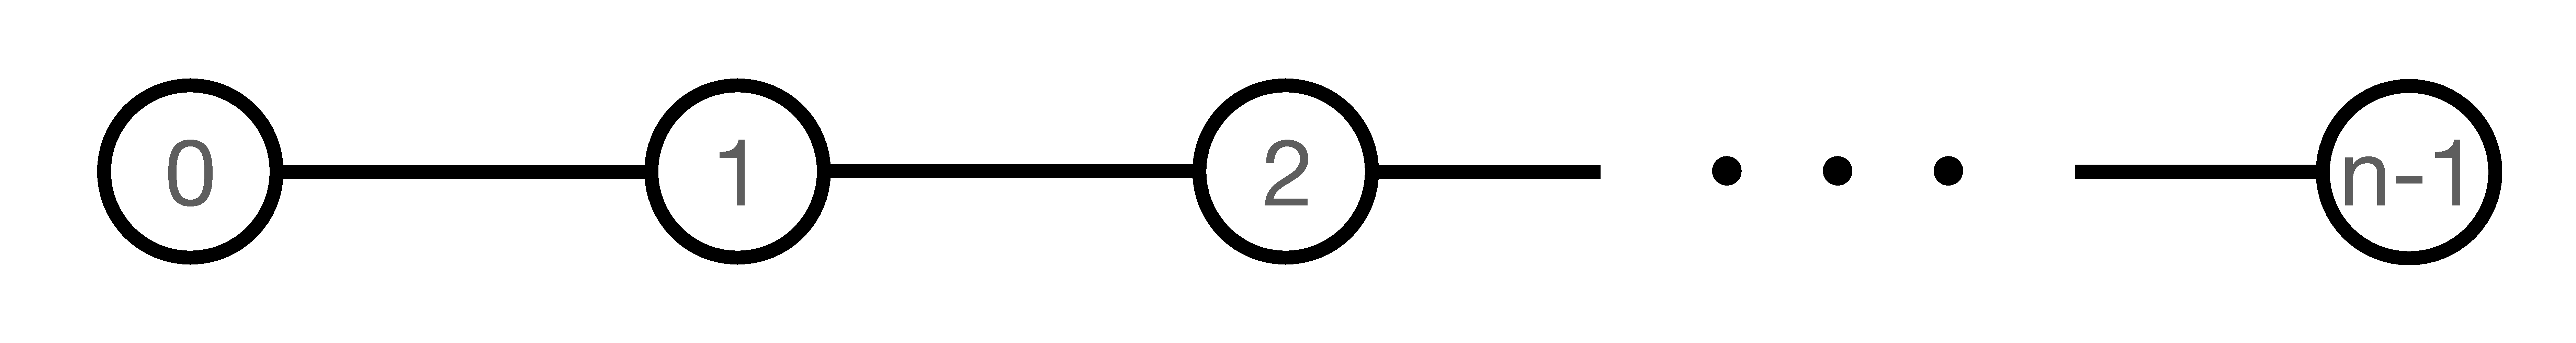
\includegraphics[width=0.8\columnwidth]{./new_figures/linear_graph.pdf}}
	\end{tabular}
	\caption{Linear graphs $G(n)$ used in this study. Nodes denote vertices of the graphs and lines are undirected edges.}
\label{fig:linear}
\end{figure}

We demonstrate the proposed algorithm in order to obtain the MDS on a series of linear graphs $G(n)$ as shown in Fig.~\ref{fig:linear}. Details of the mapping of ILP to MDS is given in Sec.~\ref{sec:methods:mds-qubo}. This type of graph is chosen because the small number of nearest-neighbor connections is more efficiently embedded into the chimera graph allowing for scaling plots to be generated when using a DWave quantum annealer. Additionally the MDS solution is known analytically, and contains both unique and degenerate solutions. In particular, the domination number for $G(n)$ is $\lceil n/3 \rceil$ while the number of MDS solutions for $n$ vertices is
\begin{align}
&1 &&\textrm{if} && n\textrm{ mod }3=0,\nonumber \\
&2\lfloor n/3 \rfloor + 1 && \textrm{if}&& n\textrm{ mod }3=1,\nonumber \\
&\lfloor n/3 \rfloor + 2 && \textrm{if} && n \textrm{ mod }3 = 2,
\end{align}
and gives the probability of randomly guessing the MDS of $G(n)$.

For even the smallest graph $G(2)$, the MDS problem is not native to the chimera graph and must be embedded. Following the hypothesis of MBL, we therefore, must look at the values of $h_i$ after embedding. The qubits then split into two groups depending on the value of $h_i$ relative to $(\textrm{max}|\{h\}| + \textrm{min}|\{h\}|) / 2$ given the set of external magnetic fields $\{h\}$ defined by a specific embedding. Further detail is given in Sec.~\ref{sec:methods:minor_embedding}. We study the effects of delaying the anneal schedule of one group of qubits over the other and present the results of this study is shown in Fig.~\ref{fig:baseline}.

For the following studies, we perform experiments on the \texttt{DW\_2000Q\_6} solver. The annealing time is set to 500$\mu$s after performing a study on various annealing times the $G(6)$ graph. The black line (offset$=0.0$) in Fig.~\ref{fig:baseline} shows results from the baseline experiment, without modification to the DWave annealing schedule, and observe improvement over random guessing (blue).

\begin{figure}
	\centering
	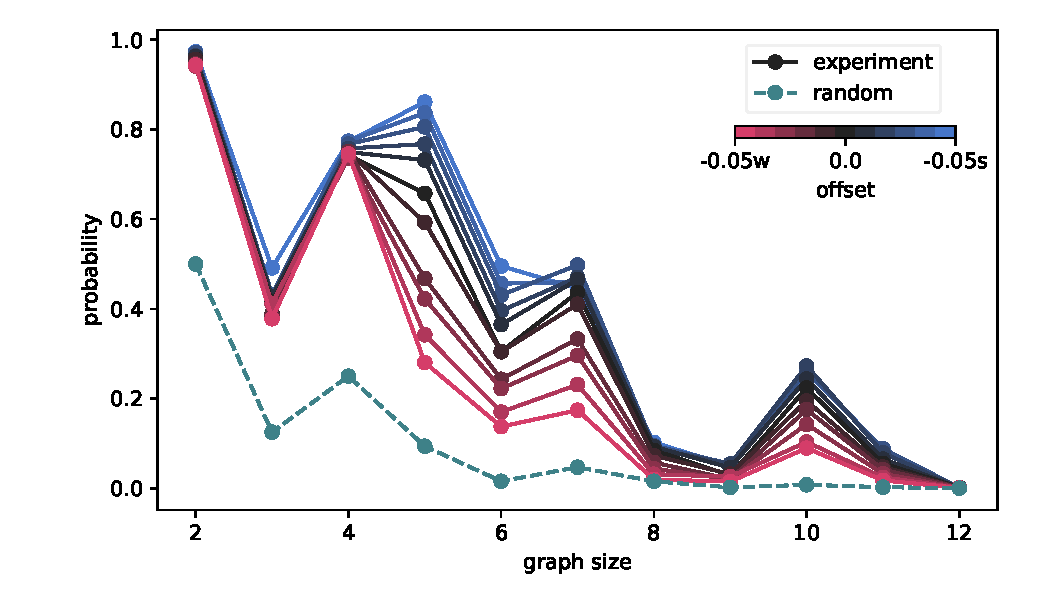
\includegraphics[width=\columnwidth]{./new_figures/DWave_scaling.pdf}
	\caption{Baseline result of DWave (black) compared to random guessing (blue). The jagged nature of random guessing reflects the degeneracy of the ground state. The legend labels the values of annealing offsets employed. A positive offsets (yellow) indicates that qubits with large values of $|h_i|$ are annealing with a delayed schedule, while negative offsets (green) delay the schedule of qubits with small values of $h_i$.}
	\label{fig:baseline}
\end{figure}

We explore one avenue towards improving the experiment results by introducing per-qubit annealing offsets into the time evolution.
The results in yellow (green) delays the annealing of qubits subject to stronger (weaker) external fields. We observe improvement (diminishment) in the experimental results when qubits subject to stronger (weaker) final external fields are delayed in the anneal schedule, in agreement with the MBL hypothesis. The phenomena is observed across different problem sizes and hints at the possibility of a generic improvement strategy.


%----------------------------------------------------------------------------------------
\subsection{Simulation Results}
%----------------------------------------------------------------------------------------
\label{sec:results:simulation}
In order to understand the effects of annealing offsets, we simulate the annealing process for the $G(2)$ graph embedded in chimera topography.
In order to shorten the simulation time, we repeat the same anneal process with a total annealing time of 1 $\mu s$ and count the number of correct ground state occurances.
The resulting ground state probability as a function of offset measured over 100,000 observations is shown in Fig.~\ref{fig:dwave1us}.

\begin{figure}
	\centering
	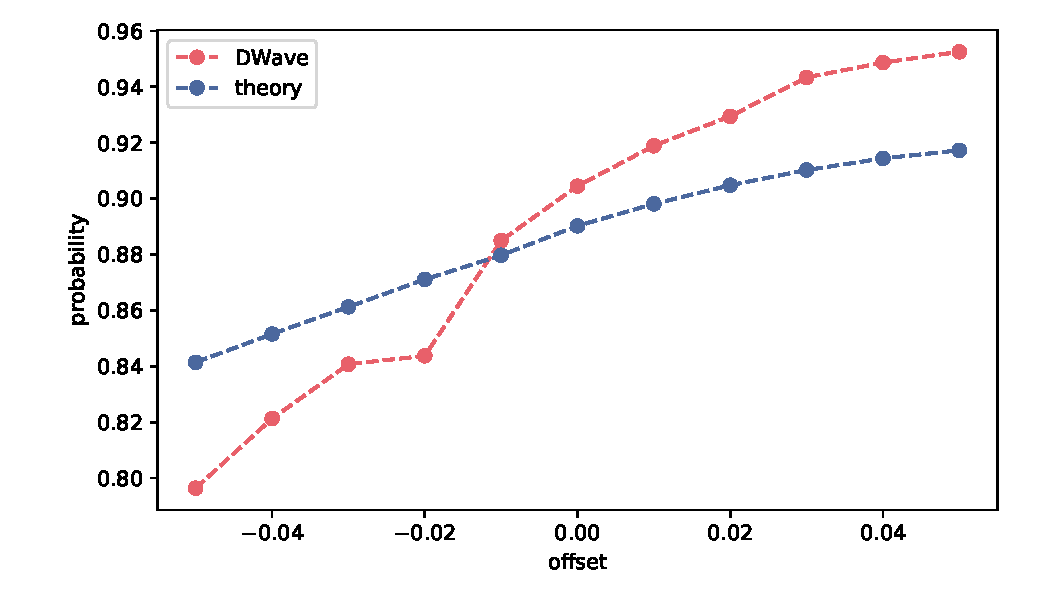
\includegraphics[width=\columnwidth]{./new_figures/NN2_offset_scaling.pdf}
	\caption{The probability of finding the MDS for $G(2)$ from DWave (orange) and results from simulation with both decoherence terms (blue).
     The machine parameters are identical to Sec.~\ref{sec:discussion:qa} with the exception of shortening the total annealing time to 1 $\mu s$ to accommodate reasonable simulation times.}
	\label{fig:dwave1us}
\end{figure}


To solve for time evolution dynamics of quantum annealing including thermal and the decoherence effects, we solve for the master equation in Lindblad form
\begin{align}
 \partial_t \rho (t) =  \frac{-i}{\hbar} [H(t) , \rho(t)] + \mathcal{L}(\rho(t), H(t))
\end{align}
where $\rho (t)$ is the density matrix at time $t$, $H(t)$ is the time-dependent Hamiltonian and $\mathcal{L}$ is the Linblad operator implementing the decoherence models.
In this work, we consider two types of decoherence models: full counting statistics and local damping.
The full counting statistics term models the global decoherence to all the qubits due to the classical reservoir.
The local damping term models the decoherence of each qubit independently.
Details of the master equation are given in Sec.~\ref{sec:methods:lindblad}.

The graph $G(2)$ has the interesting feature of having a degenerate ground state depending on whether qubit 0 or 1 is chosen to be the MDS solution.
This degeneracy is reflected in the experimental result and provides a non-trivial benchmark for our simulation.
Fig.~\ref{fig:final_state_distribution} show the final state distribution of the three lowest lying state.
The states $(0, 1, 0, 0, 0)$ and $(1, 0, 0, 1, 0)$ are the two degenerate ground states of the embedded Hamiltonian, while $(1, 1, 1, 1, 1)$ is the first excited state which yields an incorrect solution.
All other states receive negligible probability at the end of annealing.
The simulation (black) captures main features of the experimental result: 1) significant probability to populate both ground states (rather than populating only one), 2) asymmetry in ground state population due to systematic effects of offset lifting the final state degeneracy spanning approximately the correct range, 3) population of first excited state with systematically lower probability when the strong field is delayed.
The asymmetry in the ground state distribution is a result of annealing offsets lifting the ground state degeneracy. Within the broken symmetry, the non-degenerate ground state switches between the two states depending on which qubit group is delayed.
This result can be obtained by tuning three free parameters: the simulation temperature to the order of 10 milliKelvin, and the two coefficients of the two decoherence models at the order of 1 to 10 $ns$.
Additional insights of the simulation are given in Sec.~\ref{sec:methods:simulation_details}.

The resulting probability of recovering the correct solution as a function of annealing offset is given in Fig.~\ref{fig:dwave1us}.
We confirm that scaling with respect to offset from the simulation matches what is observed from experiment, and provides evidence suggesting that the improvements are related to quantum mechanics.
An additional study where an extended annealing schedule is employed in the simulation which removes systematic errors introduced by annealing offsets and effects of local damping are presented in Sec.~\ref{sec:methods:annealing-schedule}, and further supports this observation.

\begin{figure}
	\centering
	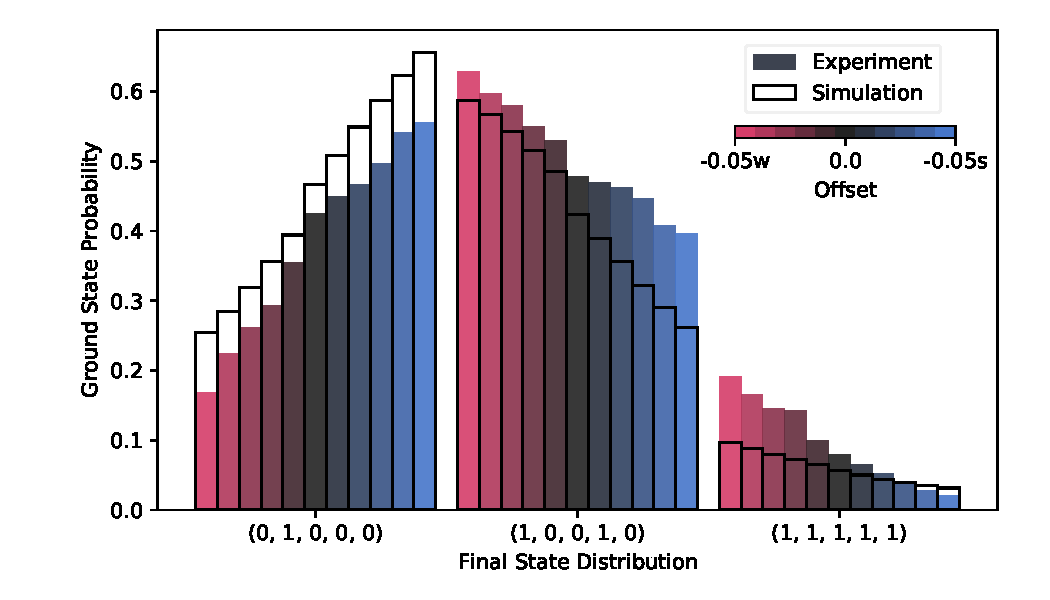
\includegraphics[width=\columnwidth]{./new_figures/final_state_distribution.pdf}
	\caption{{\color{red}I need to add dwave final state distribution here too.}}
	\label{fig:final_state_distribution}
\end{figure}

\ghissue{Decoherance study}{31}

\subsection{Final remarks}
\label{sec:results:final}
We would like to emphasize that while the annealing offsets are motivated by the MBL hypothesis, and the results also follow those expectations, we do not have definitive proof that MBL plays a crucial role.
The reason is because observations of MBL inevitably require the study of finite-size scaling, and our current simulation while being extremely thorough and explicit, is exponentially slow to evaluate making evaluations of even $G(3)$ untenable.
However, the intersection of time-dependent quantum mechanics and emergent phenomena such at MBL is an exciting direction that is pertinent to adiabatic quantum computing.


\ghissue{Conclusion}{20}




%========================================================================================
\section{METHODS}
\label{sec:methods}
%========================================================================================
%----------------------------------------------------------------------------------------
\subsection{Additional Mappings to QUBO}
\label{sec:methods:ILP-to-QUBO}
%----------------------------------------------------------------------------------------
%----------------------------------------------------------------------------------------
\subsubsection{Minimum Dominating Set Qubo}
\label{sec:methods:mds-qubo}
%----------------------------------------------------------------------------------------

The solution to the Minimum Dominating Set problem can be expressed as an integer optimization problem given by,
\begin{align}
 f(\vec x) = & \min\left(\sum_{v \in V} x_v\right),                    \\
\end{align}
subject to
\begin{align}
 & x_v + \sum_{j \in \mathcal{N}(v)} x_j \geq 1, \\
 & x_v \in \{0, 1\}
\end{align}
where $\mathcal{N}(v)$ represents the set of all direct neighbors of vertex $v$ and the dimension of the dependent variable $x$ is the number of vertices $n_V \equiv \overline{\overline{V}}$.
The problem minimizes the number of vertices in $D$ with a binary variable $\vec x = \vec \Psi_x$ encoded by single qubit, subject to the constraint that at least one vertex in $\mathcal{N}(\nu)$ is in $D$.
For each vertex in $V$ we introduce slack variables
\begin{equation}
    \vec s \in \left\{ \mathbb{Z}^{n_V} \, \middle| \, 0 \leq s_{v} \leq |\mathcal{N}(v)| \quad \forall v\in V \right\} \, ,
\end{equation}
which is related to the qubit vector $\vec \Psi_s$ by $\vec s = T_s \vec \Psi_s$, to encode the inequality constraint such that
\begin{align}
 f(\vec \Psi_x)
 =
 & \min\left(\vec 1 \cdot \vec \Psi_x \right) \, ,
\end{align}
subject to
\begin{align}
 &
 \vec \Psi_x + J \vec \Psi_x - T_s \Psi_s  - \vec 1 = 0\,,
 \\
 &
 (\vec \Psi_s)_\nu \in \{ 0, 1\}
\end{align}
where the nearest-neighbor sum is expressed by $J$ (zero diagonal and symmetric for non-directional graphs), the adjacency matrix for $G$.
The algorithm uses
\begin{equation}
    N_q = \overline{\overline{V}} + \sum_{v \in V} \log_2 \mathcal{N}(v)
\end{equation}
qubits to encode the vertices and to embed the slack variables.
Therefore, the (logical) qubit vector $\vec \Psi$ at worst scales with $n_V \log_2 n_V$ qubits for fully connected graphs.

The target QUBO in the notation of eq.~\eqref{eq:matrix_form} reads
 {\small
  \begin{align}
   Q_{xx} & = \mathbbm{1} + p\left[J^T J + J^T + J - 2 \mathrm{diag}(|J|) - \mathbbm{1} \right] \,, \\
   Q_{sx} & = - p(\mathbbm{1}+J^T)T_s\,,                                                                     \\
   Q_{ss} & = p\left[{T_s}^T T_s + 2\mathrm{diag}(|T_s|)\right]\,,                                  \\
   C      & =  p \overline{\overline{V}}\,,
  \end{align}}
where $ |M| \equiv \sum_{\nu} M_{\nu \mu}$.

%----------------------------------------------------------------------------------------
\subsubsection{Integer quadratic optimization}
\label{sec:methods:ilp:quadratic}
%----------------------------------------------------------------------------------------

Because quantum annealing is capable of solving quadratic problems, we extend the proposed algorithm to solve integer quadratic optimization problems as well such that
\begin{align}
 \vec x_0 = \mathrm{arg}\min\limits_{x}\left(\sum_{ij} x_i d_{ij} x_j + \sum_i c_i x_i\right)
\end{align}
without the introduction of auxiliary qubits.

In this case the $Q_{xx}$ component of the Qubo, eq.~\eqref{eq:qubo:components} obtains a new term
\begin{equation}
    Q_{xx} \to Q_{xx} + T_x^T d T_x \, .
\end{equation}

%----------------------------------------------------------------------------------------
\subsection{ILP on the DWave}
\label{sec:methods:ILP-on-DWave}
%----------------------------------------------------------------------------------------

%----------------------------------------------------------------------------------------
\subsubsection{Comment on ILP QUBO penalty term}
\label{sec:methods:ilp-qubo-comments}
%----------------------------------------------------------------------------------------

The minimal energy solution to eq.~\eqref{eq:initial-ip-def} and eq.~\eqref{eq:qubo-min} {\color{red}@chris what equation is this?} are exactly the same if the penalty term is larger than the energy gap of the first excited solution: $p > E_1 - E_0$.
Thus some knowledge of the problem is required.
In principle, it is possible to set the penalty term arbitrarily large, at the cost of problem resolution: large $p$-values increase the highest available energy of the system by multiples of $p$.
After normalization of the QUBO, this corresponds to decreasing the energy gap between the ground state and the first excited state.
Thus, if solvers have finite precision, one must estimate reasonable values for $p$: for large $p$ more solutions fulfill the constraints, while for small $p$, more solutions minimize the objective function.

%----------------------------------------------------------------------------------------
\subsubsection{Minor Embedding}
\label{sec:methods:minor_embedding}
%----------------------------------------------------------------------------------------
Our proposed offset strategy is motivated by the structure of the Hamiltonian being evaluated by the annealer.
As a result, details of the embedding are important. We obtain an embedding for $G(n)$ with the \texttt{embed\_qubo} function provided by the DWave Oceans Python package~\cite{dwave_oceans} under the \texttt{dwave.embedding} module.
The same embedding is used for all DWave solves of the same graph (independent of offset), and consequently the simulation solves the resulting embedded Hamiltonian for $G(2)$.
Additionally, solving the same graph as a function of offset on the exact same qubits removes (or at least keeps consistent) the systematic effects due to solving a problem on different physical qubits.
We note that comparisons between different graphs in Fig.~\ref{fig:baseline} are subject to this uncontrolled systematic.

After embedding the QUBO for $G(2)$ requires 5 qubits (an increase from 4), where by construction, qubits 0 and 3 form the qubit chain.
We confirm through brute force evaluation of the eigenvalue decomposition of the 5 qubit Hamiltonian, that the embedding provided by DWave solves the expected ILP problem for $G(2)$, with degenerate ground states at $(0, 1, 0, 0, 0)$ and $(1, 0, 0, 1, 0)$ corresponding to whether vertex 0 or 1 is chosen for the MDS solution, and $(1, 1, 1, 1, 1)$ as the first (non-degenerate) excited state where both vertex 1 and 0 are in the set yielding a valid dominating set but not the minimum dominating set.

The resulting Ising Hamiltonian has external field equal to $h = (2.75, 1.5, -1.0, -1.25, -1.0)$.
Following the offset strategy described in Sec.~\ref{sec:results:qa}, qubit(s) 0 (1, 2, 3, 4) are placed in the set with relatively stronger (weaker) final external fields.
This imbalance in the two groups may perhaps explain the reason why effects of delaying the weaker fields are more pronounced, since delaying the strong fields only differs from the baseline by a single qubit.



%----------------------------------------------------------------------------------------
\subsection{Simulation of a Quantum Annealer}
\label{sec:methods:simulation}
%----------------------------------------------------------------------------------------

%----------------------------------------------------------------------------------------
\subsubsection{The Lindblad Equation}
\label{sec:methods:lindblad}
%----------------------------------------------------------------------------------------

To solve for time evolution dynamics of quantum annealing including thermal and the decoherence effects, we solve for the master equation in Lindblad form
\begin{align}
 \partial_t \rho (t) =  \frac{-i}{\hbar} [H(t) , \rho(t)] + \sum_j (2L_j \rho(t) L_j^\dagger - \{ L^\dagger_j L_j, \rho(t) \}) ,
\end{align}
where $\rho (t)$ is the density matrix at time $t$.
$H(t)$ is the time-dependent Hamiltonian
\begin{align}
 \label{eq:annealH}
 H_{anneal}(t) & =  - \sum_i  A_i(t)\sigma^x_i                                                                      & \notag \\
 +             & \sum_{i>j} \sqrt{B_{i}(t)B_{j}(t)} J_{ij} \sigma^z_i \sigma^z_j +\sum_i B_{i}(t) h_i \sigma^z_i  , &
\end{align}
where $A_i(t)$ and $B_{i}(t)$ are site-dependent annealing schedule functions.
The site dependency takes into account of the annealing offset.
$[,]$ denotes the Lie bracket.
$L_j$ are the Lindblad operators for decoherence.
$\{, \}$ denotes the anti-commutator.

We consider two types of decoherence models: full counting statistics \cite{PhysRevE.90.022103} and local damping.
The full counting statistics term models the global decoherence to all the qubits due to the classical reservoir.
The local damping term models the decoherence of each qubit independently.
For full counting statistics, the Lindblad operator is
\begin{align}
\mathcal{L}[\rho (t)] &=& \Gamma_{fc} \sum_j   (2 S_j \rho(t) S_j^\dagger - \{ S^\dagger_j S_j, \rho(t) \}) \notag \\
&& + e^{-\beta \Delta E_j} (2 S_j^\dagger \rho(t) S_j - \{ S_j S^\dagger_j, \rho(t) \} )
\end{align}
where $j$ is the index for the inter-level spacing $\Delta E_j=E_\mu-E_\nu>0$. $S_j=|E_\nu \rangle \langle E_\mu|$ denotes the many-body lowering operator.
$\{, \}$ denotes the anti-commutator. $\Gamma = 1/T_c$ is the decoherence rate for coherence time $T_c$.
That is, due to the interaction with the classical thermal bath, there is a probability that the system hops from each higher-energy many-body state to a lower-energy many-body state.
The probability of the inverse process is given by a Boltzmann factor.
To model the local decoherence of each qubits in the non-interacting limit, we also consider the amplitude damping for non-interacting qubits.
The Lindblad operator is
\begin{align}
\mathcal{L}[\rho (t)] &=&  \Gamma_{loc} \sum_j (2L_j \rho(t) L_j^\dagger - \{ L^\dagger_j L_j, \rho(t) \} \notag \\
&& + e^{-\beta 2|h_j| }  (2L_j^\dagger \rho(t) L_j - \{ L_j L_j^\dagger, \rho(t) \}) ),
\end{align}
where $j$ is the index for qubit.
$L_j= \sigma^{+}_j=|1\rangle \langle 0|$ for $h_j>0$ and $L_j= \sigma^{-}_j=|0\rangle \langle 1|$ for $h_j<0$.
That is, each qubit is damped toward its local ground state if we ignore all the interactions.

The initial condition is the Gibbs canonical ensemble
\begin{equation}
\rho (0) =  \frac{e^{-\beta H(0)}}{\mbox{Tr}[e^{-\beta H(0)}]} ,
\end{equation}
where $\beta$ is the inverse temperature.
The probability to get the ground state at measurement is
\begin{align}
P =  \mbox{Tr} \{  \rho (t) \pi_{\mbox{gnd}} \}  ,
\end{align}
where the projection operator onto the degenerated ground states subspace is defined as $\pi_{\mbox{gnd}}=\sum_{i\in G} |\mbox{gnd}_i\rangle \langle \mbox{gnd}_i| $.
Here $\{ | \mbox{gnd}_i \rangle | i \in G \}$ forms an orthonormal basis for the degenerated ground states subspace, i.e., $\langle \mbox{gnd}_j | \mbox{gnd}_i \rangle = \delta_{ij}$.

For the simulation results presented, we set the temperature to 22.5 milliKelvin.
The coherence time for local decoherence is set to 15$ns$, and 1$ns$ for full-counting statistics.

%----------------------------------------------------------------------------------------
\subsubsection{Annealing schedule and offsets}
\label{sec:methods:annealing-schedule}
%----------------------------------------------------------------------------------------
In this section, we discuss the details of the annealing schedule with respect to the dimensionless normalized time $s$.
On DWave solvers, annealing offsets effectively advance or delay the annealing schedule of individual qubits ($B(s) \to B_i(s)$).
In Fig.~\ref{fig:anneal_schedule}, the default DWave annealing schedule is shown in black, in addition to the effects of applying negative offsets (effective time delay) to $A(s)$ and $B(s)$ in blue.
Further documentation is provided by DWave in Ref.~\cite{dwave_as, dwave_as_docu}.

\begin{figure}[htb]
 \centering
  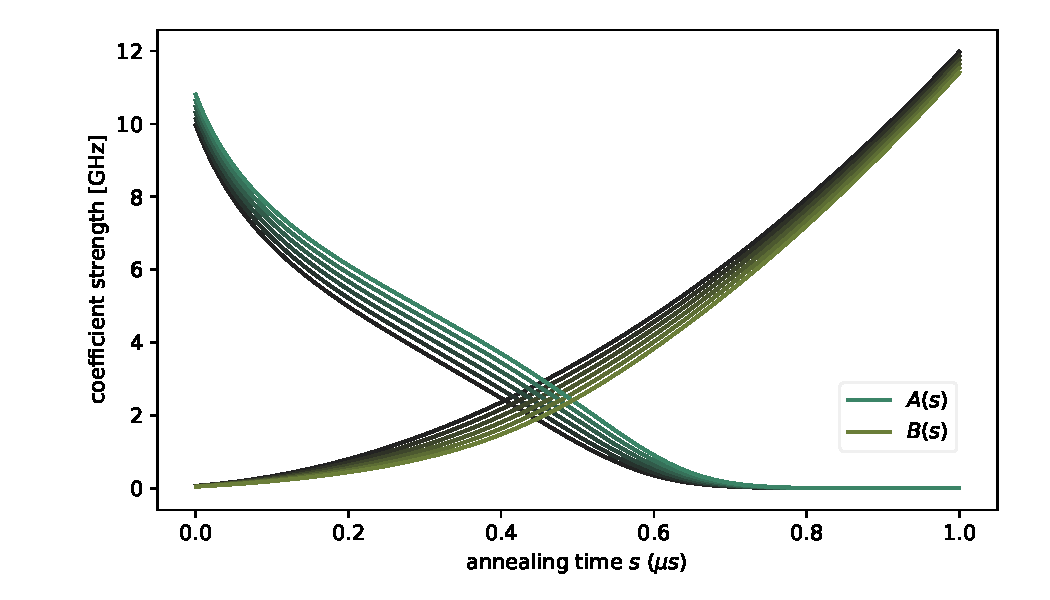
\includegraphics[width=\columnwidth]{./new_figures/anneal_schedule.pdf}
  \caption{
  Anneal schedules for amplitudes of initial Hamiltonian (top left to bottom right) and final Hamiltonian (bottom left to top right) are displayed for a complete anneal schedule.
  Different colors represent different offesets: delayed (light to dark), default (black).
 }
 \label{fig:anneal_schedule}
\end{figure}

The coefficients are nonlinear in time because the underlying control variable $c(s)$ which is designed to grow the persistent current $I_p(s)$ linearly in time.
The effective time delay is implemented by introducing an offset as $c(s) + \delta$.
As a result, systematic errors are introduced because the final values of $A(s)$ and $B(s)$ will differ for qubits with different offsets.
Additionally, the values of the coefficients are unknown outside of $s\in [0, 1]$.
We extrapolate their values by a linear extrapolation, and only employ negative offsets such that this effect only enters at the beginning of the annealing process rather than the end.

We verify that our implementation of annealing offsets on the simulator is consistent with DWave by solving the following three qubit Hamiltonian
\begin{align}
	\label{eq:offset_test_hamiltonian}
	H^{\textrm{problem}} =
	\begin{pmatrix}
		-0.25 & 1 & 0 \\
		0 & -0.25 & 0 \\
		0 & 0 & -0.25
	\end{pmatrix}
\end{align}
which has a doubly-degenerate ground state of $(0, 1, 1)$ and $(1, 0, 1)$. An annealing offset is then applied to either qubit 0 or 1, and breaks the ground state degeneracy of the system. Because of the systematic error introduced when assigning an offset to a qubit, the final Hamiltonian given by Eq.~(\ref{eq:annealH}) will have small deviations from the input problem Hamiltonian. For example, we expect a negative offset to qubit 0 to Eq.~(\ref{eq:offset_test_hamiltonian}) will yield $(1, 0, 1)$ as the unique ground state given Eq.~(\ref{eq:annealH}).

We confirm that with different combinations of annealing offsets, the degeneracy is lifted on the DWave results as expected by solving for the modified problem Hamiltonian spectrum, as well as dialing in annealing offset in the simulation of this three qubit test case.

\begin{figure}
	\centering
	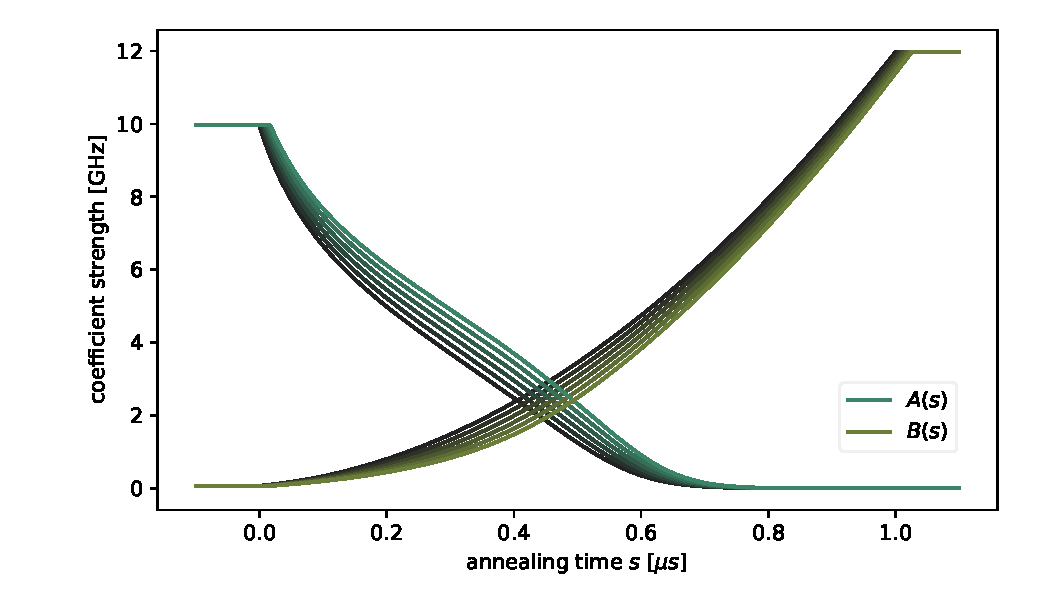
\includegraphics[width=\columnwidth]{./new_figures/anneal_schedule_extended.pdf}
	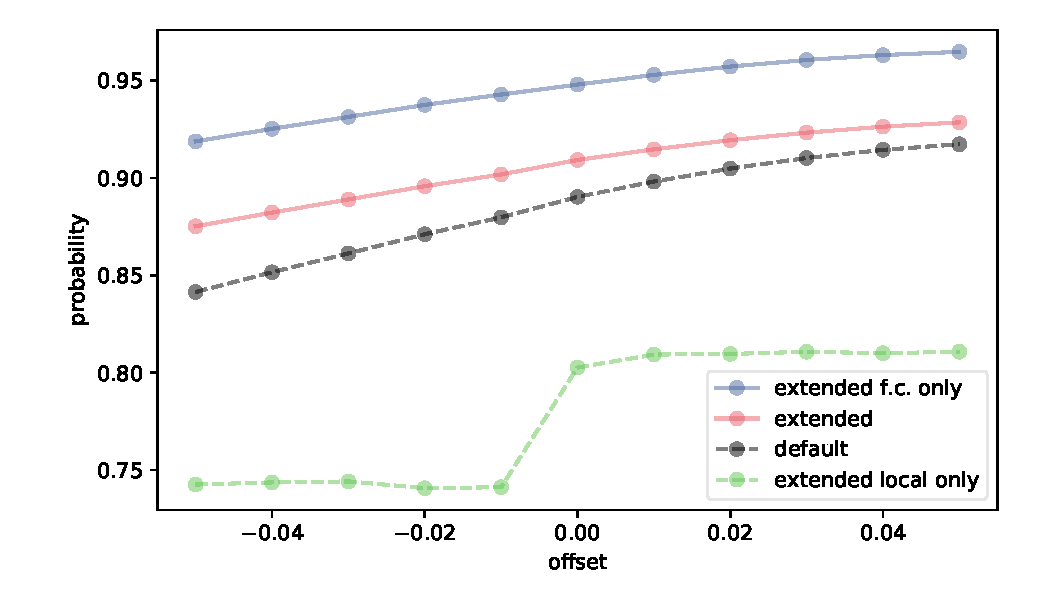
\includegraphics[width=\columnwidth]{./new_figures/NN2_offset_scaling_extended.pdf}
	\caption{{\color{red}I need to add dwave final state distribution here too.}}
	\label{fig:anneal_schedule_ext}
\end{figure}

In the simulation, we also reserve the ability to remove the systematic errors by extending the annealing schedule as shown by the red data points in Fig.~\ref{fig:anneal_schedule_ext}. With the extended schedule, all qubits start and end with the same values of $A$ and $B$ and faithfully preserves the initial and final Hamiltonians. The dependence on offset for $G(2)$ (Fig.~(\ref{fig:dwave1us})) remains the same under the extended anneal schedule (Fig.~\ref{fig:anneal_schedule_ext}), confirming that the behavior is not a systematic artifact.

The quantum system can be further idealized by including only the full-counting statistics model (blue), or local decoherence (green). We observe in both cases that the overall scaling follows the story of the MBL hypothesis. Perhaps more importantly, we observe that a simulation without local decoherence, where the relaxation is dependent on precisely the instantaneous value of $|h_i|$, exhibits the same scaling as experiment. This result suggests that our strategy for setting annealing offsets is improving the algorithm beyond the simple explanation of qubits freezing due to single-particle amplitude damping. In fact, the simulation with only amplitude damping (green) does not fully capture the results of the experiment. We observe hints of a phase transition with respect to offset (which may be thought of as some measure of disorder) when dynamical thermalization effects are removed. This is a tantalizing observation, and also is strong evidence for the inclusion of the full-counting statistics model.

It unfortunately does not make much sense to remove all decoherence models for the $G(2)$ graph for an anneal time of $1\mu s$ since all probabilities go to 1 within machine precision.

%----------------------------------------------------------------------------------------
\subsubsection{Other Simulation Details}
\label{sec:methods:simulation_details}
%----------------------------------------------------------------------------------------
To check the correctness of simulator and unit conversion, we tested a simple annealing schedule for pure transverse field, i.e. $A(s)=A(0)$ and $B(s)=0$.
The initial state is pure zero state $\rho=|00...0\rangle \langle 00...0|$.
In this case the analytical solution can be obtained for the wave function oscillation.
The time-dependent probability is $P_{0}=\cos^{2n}(s)=\cos^{2n}(t/T)$ where $n$ is the number of qubits and $T$ is the annealing time.
For annealing time $T=1/A(0)$, we expect to see perfect one-period oscillation. The energy spectrum for this system can be analytically obtained, so we also checked the Boltzmann distribution in the initial density matrix construction. The oscillation is depicted in Figure \ref{figcheck}, where the simulation matches the expected theoretical behavior.


\begin{figure}
	\centering
	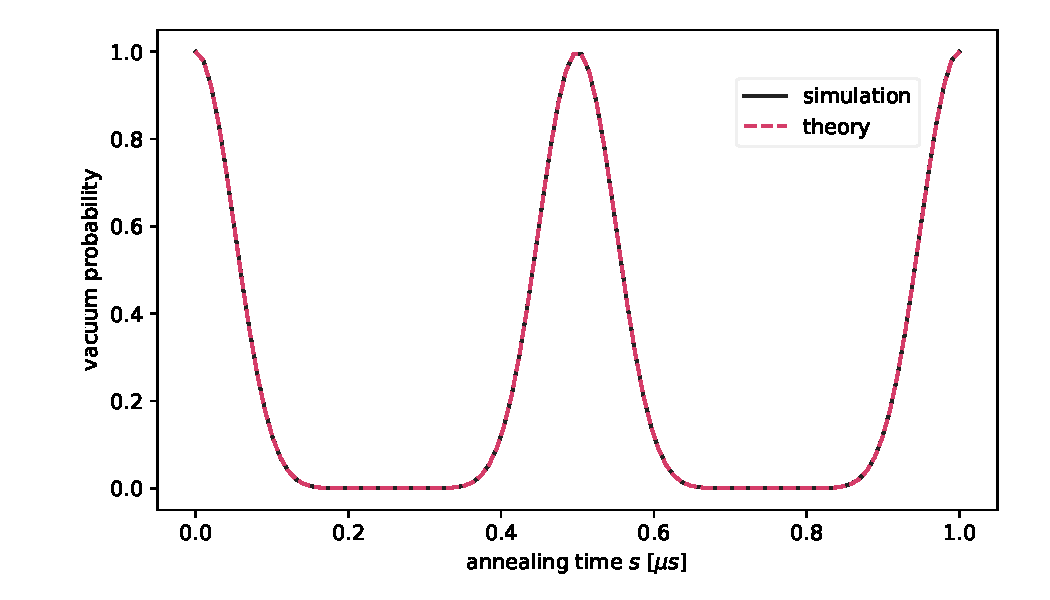
\includegraphics[width=\columnwidth]{./new_figures/vacuum_probability.pdf}
	\caption{Time dependent vacuum probability of 5 qubits system under pure transverse field.}
	\label{figcheck}
\end{figure}

Next, the simulator is applied to the $G(2)$ problem and the result is summarized in Fig.~\ref{fig:td_prob} where the time-dependent overlap with the exact Ising ground state is shown. We observe for all cases that the system undergoes what is analogous to a magnetic phase transition around $s\sim 0.4$.
After the phase transition, we are able to confirm that the system collapses to effectively a classical state in the sense that the density matrix becomes a diagonal matrix.
The steady increase in probability after the phase transition is a sensitive balance between the competing effects between full-counting statistics and local damping.
In our example, full-counting statistics is tuned to be slightly stronger, resulting in what amounts to a final thermal annealing step.
If local damping is relatively stronger, then the probability after the phase transition will slowly decrease as the system decoheres into its local ground state.
While we believe both effects are important in DWave, the experimental results are not precise enough for us to conclude which is the dominant effect.
We emphasize however, that the simulation suggests that the ground state is recovered predominantly due to the quantum phase transition.

\begin{figure}
	\centering
	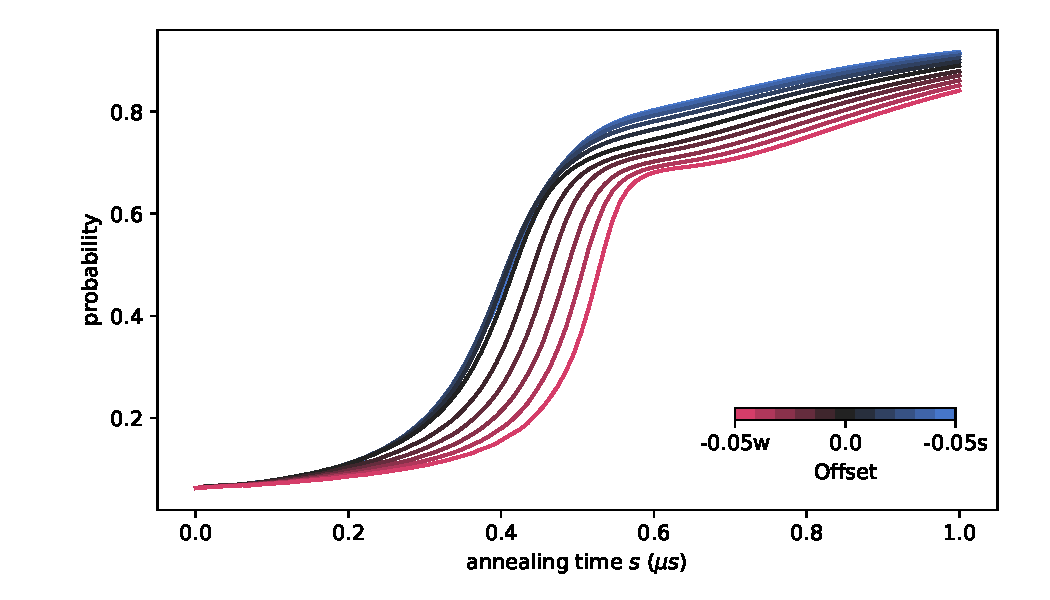
\includegraphics[width=\columnwidth]{./new_figures/time_dependent_probability.pdf}
	\caption{(Left) The time-dependent probability of resolving the ground state and (Right) the corresponding mutual information. (Top) Simulation with decoherence included and (Bottom) without decoherence.}
	\label{fig:td_prob}
\end{figure}

Finally, we comment that in order for the simulation to obtain the final state distribution shown in Fig.~\ref{fig:final_state_distribution}, effects of full-counting statistics are required.
Absent some dynamical thermalization effect, the $G(2)$ problem is too small such that at a total annealing time of 1$\mu s$, the annealing offsets lift the ground state degeneracy by an amount such that diabatic transitions are absent, and the simulation is populated predominantly by the unique ground state.
The final state distribution gives us a very sensitive observable to tune the simulation temperature, and agrees well with the experimental operating temperature.



%========================================================================================
\section{DATA AVAILABILITY}
\label{sec:open-source}
%========================================================================================

\ghissue{Data availability}{21}

%========================================================================================
\section{ACKNOWLEDGEMENTS}
%========================================================================================

\ghissue{Acknowledgements}{22}

We thank Long Gang Pang for inspiring discussions.
We thank David Johnson, Vlad Papish and the rest of D-Wave Support for answering detailed questions about the D-Wave annealer.

%========================================================================================
\section{AUTHOR CONTRIBUTIONS}
%========================================================================================

Initial idea was proposed by Chang.
All authors contributed to the design of test cases.
Calculations were performed on the D-Wave by Chang and K\"oerber.
Numerical simulations were performed by Chen, Chang, and K\"orber.
All authors contributed to writing and editing of the final manuscript.

%========================================================================================
\section{ADDITIONAL INFORMATION}
%========================================================================================

\textbf{Competing Interests:} The authors declare no competing interests.

\bibliographystyle{apsrev4-1}
\bibliography{qilp}
\ghissue{References}{24}
%========================================================================================

\end{document}
